\documentclass[12pt]{article}
\usepackage[a4paper,margin=1in]{geometry}
\usepackage[T1]{fontenc}
\usepackage[utf8]{inputenc}
\usepackage{mathptmx}
\usepackage{amsmath,amssymb}
\usepackage{graphicx}
\usepackage{float}
\usepackage[hang,flushmargin]{footmisc}
\usepackage{caption}
\usepackage{titlesec}
\usepackage{setspace}
\usepackage{xurl}
\urlstyle{same}
\usepackage[colorlinks=true,linkcolor=black,citecolor=black,urlcolor=black]{hyperref}

\onehalfspacing
\setlength{\parindent}{0.5in}
\setlength{\emergencystretch}{3em}

% ---- headings as in the journal: Roman numerals, centered bold; lettered subsections ----
\renewcommand{\thesection}{\Roman{section}}
\renewcommand{\thesubsection}{\Alph{subsection}}
\titleformat{\section}{\normalfont\bfseries\centering}{\thesection.}{0.5em}{}
\titleformat{\subsection}{\normalfont\bfseries}{\thesubsection.}{0.5em}{}
\titlespacing*{\section}{0pt}{18pt}{6pt}
\titlespacing*{\subsection}{0pt}{12pt}{4pt}
\captionsetup{labelsep=period,labelfont=bf,textfont=bf,justification=raggedright,singlelinecheck=false,skip=6pt}
\captionsetup[figure]{position=top}

\title{Bitcoin Is Not Money: Why Fixed Supply Fails in a Modern Economy}
\author{Agisilaos Papadogiannis\thanks{Independent Researcher (PhD, MBA). \textit{Correspondence:} apapadogiannis@gmail.com. \textit{ORCID:} 0009-0002-7753-7052. Forthcoming in \textit{Asian Economics Letters}. Replication code and data: \url{https://github.com/apapadogiannis/bitcoin-is-not-money}, archived at \url{https://doi.org/10.5281/zenodo.24249917}.}}
\date{November 2026}

\graphicspath{{../figures/}}
\begin{document}
\maketitle

\begin{abstract}
\noindent This paper asks whether a hard-capped monetary base such as Bitcoin's can serve as money in a growing, credit-based economy, with Asia as the reference case. Using the quantity identity and a stylized illustration, it shows that fixed supply forces adjustment through persistent deflation or velocity growth, raising real debt burdens. The policy implication is that Bitcoin should be treated as a store-of-value asset rather than a monetary anchor.
\end{abstract}

\noindent\textbf{Keywords:} Bitcoin, Monetary elasticity, Deflation.

\noindent\textbf{JEL Classifications:} E31, E42, E51

\section{Introduction}

Asia is the region where the question of whether Bitcoin can function as money is least academic. The Chainalysis Global Crypto Adoption Index ranks 151 countries by the value of cryptocurrency received on-chain, weighted by purchasing power and population, so that it measures how widely ordinary residents use crypto rather than the dollar volume traded. In its 2025 edition, India ranks first; Vietnam, Indonesia, and the Philippines are in the top ten; and the value received in Asia-Pacific grew by 69\% in the year to June 2025 (Chainalysis, 2025). The same economies are also among the fastest-growing in the world: the IMF projects real growth of 6.6\% in 2025 and 6.2\% in 2026 in India, and of 6.5\% and 5.6\% in Vietnam, while inflation in emerging Asia is expected to stay below target at 1.6\% in 2025 and 2.0\% in 2026 (IMF, 2025). Figure 1 juxtaposes the two facts: adoption is concentrated where trend growth is highest, which is where a fixed monetary base would be most deflationary.

International institutions have drawn a clear line. The IMF's policy framework advises members not to grant crypto assets legal-tender status, because doing so would weaken monetary sovereignty and the transmission of monetary policy (IMF, 2023); the joint IMF--FSB synthesis paper endorses the same position (IMF \& FSB, 2023); and the BIS argues that crypto is structurally unsuited to serve as the foundation of a monetary system (BIS, 2022). An IMF survey of 34 Asia-Pacific economies finds that private crypto adoption is itself motivating central bank digital currency (CBDC) initiatives in the region (IMF, 2022). What these institutions state as policy, this paper derives from an accounting identity.

\begin{figure}[!htbp]
\centering
\caption{Output growth and cryptocurrency adoption in selected Asian economies}
\label{fig:1}
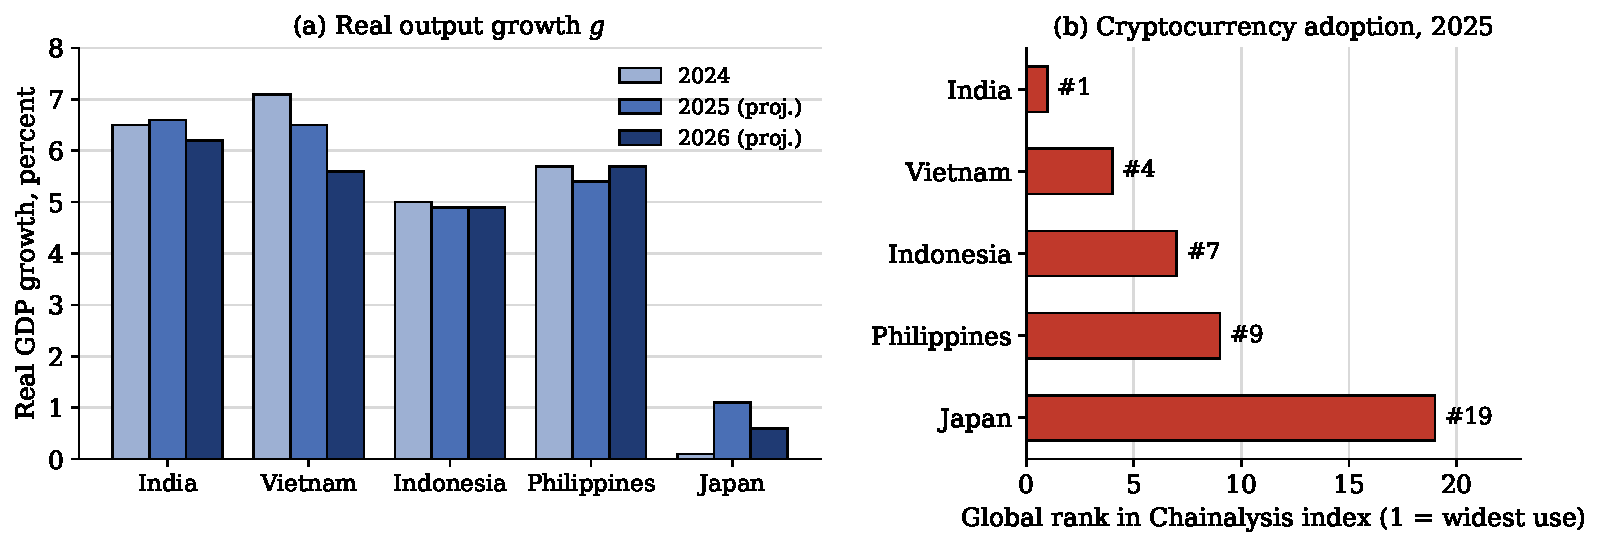
\includegraphics[width=0.98\textwidth]{fig1_growth_adoption.pdf}
\par\smallskip
\begin{minipage}{\textwidth}\footnotesize
\emph{Notes:} Panel (a) shows real GDP growth (\%) for 2024 (actual) and 2025--2026 (projections) from IMF (2025), Annex Table 1.1; data for India are on a fiscal-year basis. Panel (b) shows each economy's overall rank among 151 countries in the 2025 Chainalysis Global Crypto Adoption Index (Chainalysis, 2025), where 1 denotes the most widespread use by residents (see text for the index definition). Economies shown are those with a published rank in both sources. By Equation (3), the growth rates in Panel (a) equal the steady-state deflation rates that a fixed base with stable velocity would impose.
\end{minipage}
\end{figure}

Three strands of literature bear on the question. The first concerns Bitcoin's design. Bitcoin's monetary base is intentionally fixed: issuance is embedded in code and total supply is capped at 21 million coins, without discretionary adjustment (Nakamoto, 2008; Narayanan et al., 2016). Advocates treat this as a strength that insulates the currency from inflationary finance and political discretion (Ammous, 2018). The second strand concerns the functions of money and the case for elastic supply (BIS, 2022; Friedman, 1960). Against that benchmark, Bitcoin's volatility limits its usefulness as a medium of exchange and unit of account (Yermack, 2013), it resembles synthetic commodity money with an inelastic base (Selgin, 2015), and fixed supply creates frictions for credit formation and contracting (Schilling \& Uhlig, 2019). The third strand is the macroeconomics of deflation: with nominal debt and collateral, a falling price level raises real debt burdens and can trigger self-reinforcing balance-sheet stress (Bernanke, 1995; Eggertsson \& Krugman, 2012; Fisher, 1933), and deflations tied to financial distress have been especially costly (Borio et al., 2015; Eichengreen, 1996).

These strands have not been connected. The Bitcoin literature debates volatility, adoption, and security; the deflation literature studies fiat economies in which the money stock can respond. What is missing is an account of what a hard-capped base implies for a growing economy through the deflation channel, and an assessment of that implication for the region where adoption is fastest. This paper fills that gap. Its contribution is a compact accounting result, not a new behavioral model: under fixed supply, sustained growth must be absorbed by persistent deflation or persistent velocity growth, and neither margin is a policy instrument.

The approach is deliberately minimal. From the quantity identity, the paper derives the long-run price path implied by a fixed base, illustrates it with a stylized calibration, and examines the two escape routes invoked by Bitcoin advocates: rising velocity and benign deflation. The hypothesis is that neither route is reliable, and the results support it. With stable velocity, output growth at rate $g$ maps one-for-one into deflation at rate $g$. With variable velocity, price stability requires velocity to grow persistently at the rate of output, which settlement frictions and hoarding incentives make unlikely. A corollary is that monetary expansion should not be equated with inflation.

The remainder of the paper is organized as follows. Section II sets out the framework and the fixed-supply constraint. Section III reports the results. Section IV discusses elastic money and Bitcoin's role as an asset. Section V concludes with policy implications and limitations.

\section{Framework: The Quantity Identity and the Fixed-Supply Constraint}

Money must serve three functions: as a \emph{medium of exchange}, a \emph{unit of account}, and a \emph{store of value}. In modern economies, nominal contracts, balance-sheet leverage, and credit intermediation make the price level and the real burden of debt central to macroeconomic coordination (Fisher, 1933; Keynes, 1936). A convenient identity makes the basic constraint transparent:

\begin{equation}
M_{t} V_{t} = P_{t} Y_{t}
\end{equation}
\noindent where $M_{t}$ is the nominal money stock, $V_{t}$ is velocity,\footnote{Velocity is the number of times a unit of money is spent on final output per period, defined residually as $V_{t} = P_{t}Y_{t}/M_{t}$; higher velocity means the same money stock supports more nominal spending.} $P_{t}$ is the price level, and $Y_{t}$ is real output (Fisher, 1911). Equation (1) is an accounting identity, not a behavioral theory.\footnote{The identity holds by construction; it becomes informative once one variable is restricted, here the money stock.} It nonetheless clarifies the channels through which a monetary regime accommodates real growth: by expanding nominal liquidity, by raising velocity, or by allowing prices to fall. Fiat systems are designed to provide this elasticity (BIS, 2022; Friedman, 1960; Rogoff, 2017). Bitcoin, by contrast, removes discretionary supply adjustment at the base layer.\footnote{The ``base layer'' is the Bitcoin protocol itself; payment networks built on top of it cannot create additional units of the asset.}

Under a hard cap, the number of coins is bounded by the protocol regardless of output growth driven by productivity, population, or innovation. Taking logs and first differences of equation (1) gives the inflation decomposition:

\begin{equation}
\Delta \ln P_{t} = \Delta \ln M_{t} + \Delta \ln V_{t} - \Delta \ln Y_{t}
\end{equation}

Under a fixed-supply regime and stable long-run velocity ($\Delta \ln M_{t} = 0$ and $\Delta \ln V_{t} = 0$), it follows immediately that:

\begin{equation}
\Delta \ln P_{t} = - \Delta \ln Y_{t}
\end{equation}

If $Y_{t}$ rises persistently while $M_{t}$ cannot adjust, persistent deflation is the default adjustment unless velocity increases persistently (Fisher, 1911; Friedman \& Schwartz, 1963). This matters because deflation is not a neutral outcome in economies with nominal debt and collateralized finance: a falling price level raises real debt burdens, tightens collateral constraints, and can trigger self-reinforcing balance-sheet stress, the debt-deflation mechanism\footnote{Debt deflation: because most debt is fixed in nominal terms, a falling price level raises the real value of what borrowers owe, prompting distressed sales that push prices down further (Fisher, 1933).} (Bernanke, 1995; Eggertsson \& Krugman, 2012; Fisher, 1933), while nominal rigidities\footnote{Nominal rigidities are frictions that prevent wages and prices from adjusting downward quickly, so that deflationary pressure shows up in output and employment rather than in lower prices.} amplify unemployment and reduce investment during downturns (Akerlof \& Shiller, 2009; Keynes, 1936). Because velocity is not a policy instrument, adjustment tends to shift to the price level (Borio et al., 2015; von Peter, 2005). Section III quantifies this and tests the two proposed escape routes.

\section{Results: Deflation Under Fixed Supply and the Limits of Adjustment}

\subsection{The stylized deflation path}

To isolate the mechanism, assume a hard-capped monetary base and stable long-run velocity: $M_{t} = \bar{M}$ and $V_{t} = \bar{V}$. If real output grows as $Y_{t} = Y_{0}e^{gt}$ with $g > 0$, substitution into equation (1) yields the implied price-level path:

\begin{equation}
P_{t} = \frac{\bar{M} \bar{V}}{Y_{0} e^{gt}} = P_{0} e^{- gt}
\end{equation}
\noindent where $P_{0} = \bar{M}\bar{V}/Y_{0}$. Under fixed supply and stable velocity, sustained growth maps into sustained deflation at rate $g$ (Fisher, 1911; Friedman \& Schwartz, 1963). Figure 2 illustrates the path. Read against Figure 1, this calibration is not exotic: for India or Vietnam, $g$ of 5--7\% would imply a price level falling by roughly half every 10--14 years.

\begin{figure}[!htbp]
\centering
\caption{Stylized price-level path under a fixed monetary base}
\label{fig:2}
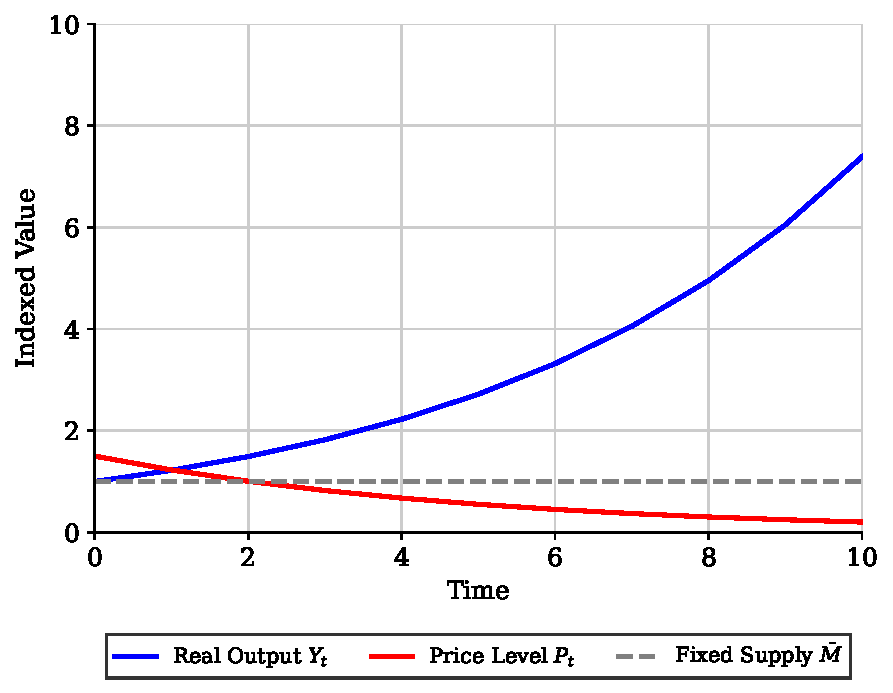
\includegraphics[width=0.68\textwidth]{fig2_price_path.pdf}
\par\smallskip
\begin{minipage}{\textwidth}\footnotesize
\emph{Notes:} The figure plots indexed real output $Y_{t}$ (blue, rising at a constant rate $g$), the fixed money stock $\bar{M}$ (dashed), and the price level $P_{t}$ (red) implied by Equation (4) with constant velocity. Time and values are stylized and chosen for visualization purposes; the qualitative result, exponential deflation at rate $g$, does not depend on the parameters.
\end{minipage}
\end{figure}

More generally, if velocity is allowed to vary while the monetary base remains fixed, the growth-rate condition becomes:

\begin{equation}
\Delta \ln P_{t} = \Delta \ln V_{t} - \Delta \ln Y_{t}
\end{equation}

Hence, price stability ($\Delta \ln P_{t} \approx 0$) requires velocity to grow at roughly the same rate as real output. In principle, adoption waves or automation (for example, high-frequency machine-to-machine payments)\footnote{Machine-to-machine payments are automated, high-frequency payments initiated by software agents; in principle, they raise the number of transactions per unit of money, that is, velocity.} could raise velocity. The economic question is whether such increases are persistent and large enough to offset growth, given that velocity is shaped by payment frictions, settlement capacity, and behavioral incentives (Narayanan et al., 2016; Schilling \& Uhlig, 2019; Selgin, 2015).

\subsection{Can velocity or deflation compensate?}

A common defense of Bitcoin's fixed supply is that economic growth can be accommodated through higher velocity. Equation (5) makes the requirement explicit, and it is demanding. In the Bitcoin network, confirmation times, mempool congestion, and incentive structures limit effective circulation, while hoarding reduces turnover under expectations of appreciation (Narayanan et al., 2016). Expected deflation therefore lowers velocity exactly when higher velocity is needed, working against the escape route rather than for it.

A second argument holds that deflation is desirable: if prices fall, money gains value and savers are rewarded. In economies with nominal contracts and debt, however, sustained deflation is destabilizing (Fisher, 1933; Keynes, 1936): consumers delay purchases, real debt burdens rise, investment is postponed, and nominal wages resist adjustment. Figure 3 summarizes the loop. Historical experience, including the interwar gold standard, links deflation to weak demand, unemployment, and financial stress (Bernanke, 1995; Borio et al., 2015; Eichengreen, 1996). For Asian emerging markets, where inflation is already below target and private debt-at-risk has risen (IMF, 2025), the loop would start from an unfavorable position.

\begin{figure}[!htbp]
\centering
\caption{Deflationary feedback loop in a fixed-supply economy}
\label{fig:3}
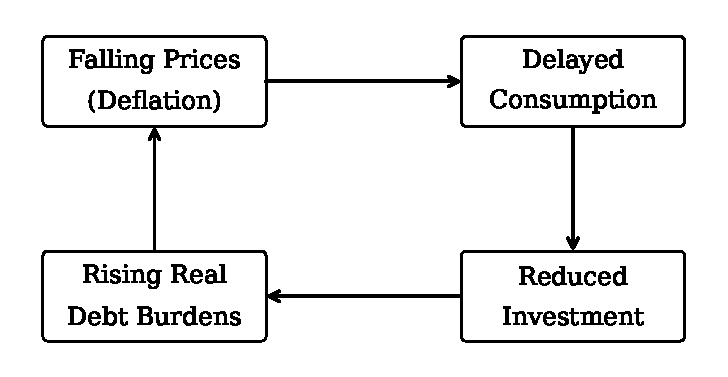
\includegraphics[width=0.62\textwidth]{fig3_deflation_loop.pdf}
\par\smallskip
\begin{minipage}{\textwidth}\footnotesize
\emph{Notes:} The diagram is schematic and traces the debt-deflation mechanism of Section II: a falling price level delays consumption, reduces investment, and raises the real value of nominal debt, which further weakens demand and prices. ``Debt burdens'' refers to real (inflation-adjusted) debt obligations, which rise when the price level falls.
\end{minipage}
\end{figure}

Accordingly, neither reliance on rising velocity nor acceptance of persistent deflation provides a robust substitute for supply elasticity in a monetary system intended to support a growing, credit-based economy.

\section{Discussion}

The results also clarify a common confusion. Bitcoin advocates often treat any expansion of the money supply as monetary destruction. Debasement is a reduction in the metallic content or backing of the monetary unit; inflation is a sustained loss of its purchasing power. Reducing the dollar's gold content from roughly one-twentieth to one thirty-fifth of an ounce in 1934 was a debasement in this sense, conventionally termed a devaluation against gold (Bordo \& Kydland, 1995); whether it produced inflation depended on real-side conditions. Equation (2) states the point directly: monetary expansion ($\Delta \ln M_{t} > 0$) does not imply inflation ($\Delta \ln P_{t} > 0$). Inflation requires that nominal spending growth, $\Delta \ln M_{t} + \Delta \ln V_{t}$, persistently exceed real output growth (Fisher, 1911; Friedman \& Schwartz, 1963). This is why modern economies deliberately target low, stable inflation: a modest positive inflation target stabilizes expectations, allows real wages to fall without cuts to nominal pay when demand weakens, which limits job losses, and lowers real interest rates in downturns (Eggertsson \& Krugman, 2012; Rogoff, 2017). Bitcoin has no comparable instrument: its base cannot expand in response to shocks or shifts in money demand (Schilling \& Uhlig, 2019; Selgin, 2015).

None of this denies that Bitcoin has economic value. It is a scarce digital asset, it enables decentralized value transfer without trusted intermediaries, and it can hedge against discretionary monetary expansion (Schilling \& Uhlig, 2019; Selgin, 2015). But a currency must be sufficiently stable to serve as a unit of account, sufficiently elastic to accommodate shifts in money demand, and sufficiently integrated with credit to support long-term nominal commitments (Yermack, 2013). Bitcoin falls short on each dimension: its base is fixed, its market value is volatile, and long-maturity nominal contracts are hard to write in a deflation-prone unit. Bitcoin is therefore best understood as a store-of-value asset with a transparent issuance rule and a tamper-resistant settlement layer, a role distinct from serving as the monetary foundation of a modern economy.

\section{Conclusion}

This paper provides a concise macroeconomic statement of the fixed-supply constraint. Combining the quantity identity with a stylized illustration, it shows that if real output grows while the monetary base is hard-capped, long-run accommodation must occur through persistent deflation or persistent increases in velocity. Both margins fail as a monetary foundation for a growing, credit-based economy: deflation raises real debt burdens and amplifies balance-sheet stress, while velocity is not a policy instrument and is constrained by settlement frictions and behavioral incentives.

Three policy implications follow, and they are sharpest for Asia. First, the IMF and FSB position against granting crypto assets legal-tender status (IMF, 2023; IMF \& FSB, 2023) has a precise macroeconomic rationale: in the region's high-growth economies, anchoring money to a fixed base would convert trend growth of 5--7\% into deflation of the same order. Second, the appropriate regulatory frame for Bitcoin is that of an asset class (prudential, conduct, and tax rules), not that of a currency, consistent with the regulatory direction in the region, for example Vietnam's 2025 Law on Digital Technology Industry, which recognizes crypto assets as a class of property distinct from legal currency (National Assembly of Vietnam, 2025). Third, the demand behind Asian adoption (remittances, savings, and payments where banking access is thin) is real and would be better met by elastic digital instruments, such as CBDCs or well-regulated stablecoins, than by a hard-capped asset.

Four limitations should be noted. First, the argument is an accounting one: it establishes what a fixed supply implies for the price level, not how quickly or how severely that implication would bind in practice. Second, velocity is treated as bounded by frictions rather than modeled explicitly; a technology that raised velocity persistently at the rate of output would weaken the conclusion. Third, the analysis assumes full adoption, whereas the empirically relevant case in Asia is partial adoption alongside fiat money, which raises further questions of currency substitution and capital-flow volatility. Fourth, the regional evidence in Figure 1 is descriptive rather than causal. Each caveat narrows the scope of the claim, but none reverses it: hard-capped supply restricts Bitcoin's ability to function as money at the macroeconomic level, particularly in economies where trend growth and financial deepening make monetary elasticity central to stabilization.

\section*{Data and Replication Statement}

Figure 1 uses published data from IMF (2025), Annex Table 1.1, and Chainalysis (2025), as reported in the figure notes. Figures 2 and 3 are stylized and fully reproducible from the equations in the text. Replication code and the data underlying Figure 1 are available at \url{https://github.com/apapadogiannis/bitcoin-is-not-money} and archived on Zenodo (\url{https://doi.org/10.5281/zenodo.24249917)}.

\section*{CRediT Statement}

The author: Conceptualization; Formal analysis; Writing -- original draft; Writing -- review \& editing; Visualization.

\textbf{Disclaimer}

This research was conducted independently and without funding, review, or endorsement. The views expressed are solely those of the author and do not represent any institutional position. This paper is for informational and academic purposes only and does not constitute financial, investment, tax, or legal advice, nor a recommendation to buy or sell any financial instrument. Any illustrative data used are from publicly available sources.

\section*{Disclaimer}

This research was conducted independently and without funding, review, or endorsement. The views expressed are solely those of the author and do not represent any institutional position. This paper is for informational and academic purposes only and does not constitute financial, investment, tax, or legal advice, nor a recommendation to buy or sell any financial instrument. Any illustrative data used are from publicly available sources.

\section*{References}
\begingroup
\small
\setlength{\parindent}{-1.5em}\setlength{\leftskip}{1.5em}\setlength{\parskip}{0.3em}\sloppy

Akerlof, G. A., \& Shiller, R. J. (2009). \emph{Animal spirits: How human psychology drives the economy, and why it matters for global capitalism}. Princeton University Press.

Ammous, S. (2018). \emph{The Bitcoin standard: The decentralized alternative to central banking}. Wiley.

Bank for International Settlements (BIS). (2022). The future monetary system. In \emph{Annual Economic Report 2022} (Chapter III). \url{https://www.bis.org/publ/arpdf/ar2022e3.htm}

Bernanke, B. S. (1995). The macroeconomics of the Great Depression: A comparative approach. \emph{Journal of Money, Credit and Banking, 27}(1), 1--28.

Bordo, M. D., \& Kydland, F. E. (1995). The gold standard as a rule: An essay in exploration. \emph{Explorations in Economic History, 32}(4), 423--464.

Borio, C., Erdem, M., Filardo, A., \& Hofmann, B. (2015). The costs of deflations: A historical perspective. \emph{BIS Quarterly Review}, March, 31--54.

Chainalysis. (2025). \emph{The 2025 Global Crypto Adoption Index}. \url{https://www.chainalysis.com/blog/2025-global-crypto-adoption-index/}

Eggertsson, G. B., \& Krugman, P. (2012). Debt, deleveraging, and the liquidity trap: A Fisher-Minsky-Koo approach. \emph{The Quarterly Journal of Economics, 127}(3), 1469--1513.

Eichengreen, B. (1996). \emph{Golden fetters: The gold standard and the Great Depression, 1919--1939}. Oxford University Press.

Fisher, I. (1911). \emph{The purchasing power of money: Its determination and relation to credit, interest and crises}. Macmillan.

Fisher, I. (1933). The debt-deflation theory of great depressions. \emph{Econometrica, 1}(4), 337--357.

Friedman, M. (1960). \emph{A program for monetary stability}. Fordham University Press.

Friedman, M., \& Schwartz, A. J. (1963). \emph{A monetary history of the United States, 1867--1960}. Princeton University Press.

International Monetary Fund (IMF). (2022). \emph{Towards central bank digital currencies in Asia and the Pacific: Results of a regional survey} (FinTech Note 2022/009). International Monetary Fund. \url{https://doi.org/10.5089/9798400221521.063}

International Monetary Fund (IMF). (2023). \emph{Elements of effective policies for crypto assets} (Policy Paper 2023/004). International Monetary Fund. \url{https://doi.org/10.5089/9798400234392.007}

International Monetary Fund (IMF). (2025). \emph{Regional economic outlook: Asia and Pacific, October 2025: Navigating trade headwinds and rebalancing growth}. International Monetary Fund. \url{https://www.imf.org/en/publications/reo/apac/issues/2025/10/24/regional-economic-outlook-for-asia-and-pacific-october-2025}

International Monetary Fund \& Financial Stability Board (IMF \& FSB). (2023). \emph{IMF--FSB synthesis paper: Policies for crypto-assets}. Financial Stability Board. \url{https://www.fsb.org/2023/09/imf-fsb-synthesis-paper-policies-for-crypto-assets/}

Keynes, J. M. (1936). \emph{The general theory of employment, interest and money}. Macmillan.

Nakamoto, S. (2008). \emph{Bitcoin: A peer-to-peer electronic cash system}. \url{https://bitcoin.org/bitcoin.pdf}

Narayanan, A., Bonneau, J., Felten, E., Miller, A., \& Goldfeder, S. (2016). \emph{Bitcoin and cryptocurrency technologies: A comprehensive introduction}. Princeton University Press.

National Assembly of Vietnam. (2025). \emph{Law on Digital Technology Industry} (Law No. 71/2025/QH15). \url{https://thuvienphapluat.vn/van-ban/EN/Cong-nghe-thong-tin/Law-71-2025-QH15-Digital-Technology-Industry/668801/tieng-anh.aspx}

Rogoff, K. (2017). \emph{The curse of cash}. Princeton University Press.

Schilling, L. M., \& Uhlig, H. (2019). Some simple Bitcoin economics. \emph{Journal of Monetary Economics, 106}, 16--26.

Selgin, G. (2015). Synthetic commodity money. \emph{Journal of Financial Stability, 17}, 92--99.

von Peter, G. (2005). \emph{Debt-deflation: Concepts and a stylised model} (BIS Working Paper No. 176). Bank for International Settlements.

Yermack, D. (2013). \emph{Is Bitcoin a real currency? An economic appraisal} (NBER Working Paper No. 19747). National Bureau of Economic Research.

\endgroup
\end{document}
